% !TEX TS-program = pdflatex
% !TEX encoding = UTF-8 Unicode

% This is a simple template for a LaTeX document using the "article" class.
% See "book", "report", "letter" for other types of document.

\documentclass[12pt,a4paper,titlepage]{article} % use larger type; default would be 10pt

\usepackage[utf8x]{inputenc} % set input encoding (not needed with XeLaTeX)

%%% Examples of Article customizations
% These packages are optional, depending whether you want the features they provide.
% See the LaTeX Companion or other references for full information.

%%% PAGE DIMENSIONS
\usepackage{geometry} % to change the page dimensions
\geometry{a4paper} % or letterpaper (US) or a5paper or....
% \geometry{margin=2in} % for example, change the margins to 2 inches all round
% \geometry{landscape} % set up the page for landscape
%   read geometry.pdf for detailed page layout information

\usepackage{graphicx} % support the \includegraphics command and options
\usepackage{wrapfig}

% \usepackage[parfill]{parskip} % Activate to begin paragraphs with an empty line rather than an indent

%%% PACKAGES
\usepackage{booktabs} % for much better looking tables
\usepackage{array} % for better arrays (eg matrices) in maths
\usepackage{paralist} % very flexible & customisable lists (eg. enumerate/itemize, etc.)
\usepackage{verbatim} % adds environment for commenting out blocks of text & for better verbatim
\usepackage{subfig} % make it possible to include more than one captioned figure/table in a single float
% These packages are all incorporated in the memoir class to one degree or another...
\usepackage[ngerman]{babel}
\usepackage{pifont} %for symbols (i.e. arrows)

%%redifine of emph, see http://tex.stackexchange.com/questions/6754/what-is-the-canonical-way-to-redefine-the-emph-command
\makeatletter
\DeclareRobustCommand{\em}{%
  \@nomath\em \if b\expandafter\@car\f@series\@nil
  \normalfont \else \bfseries \fi}
\makeatother

%%% HEADERS & FOOTERS
\usepackage{fancyhdr} % This should be set AFTER setting up the page geometry
\pagestyle{fancy} % options: empty , plain , fancy
\renewcommand{\headrulewidth}{0pt} % customise the layout...
\lhead{}\chead{}\rhead{}
\lfoot{}\cfoot{\thepage}\rfoot{}

%%% SECTION TITLE APPEARANCE
\usepackage{sectsty}
\allsectionsfont{\sffamily\mdseries\upshape} % (See the fntguide.pdf for font help)
% (This matches ConTeXt defaults)

%%% ToC (table of contents) APPEARANCE
%\usepackage[nottoc,notlof,notlot]{tocbibind} % Put the bibliography in the ToC
%\usepackage[titles,subfigure]{tocloft} % Alter the style of the Table of Contents
%\renewcommand{\cftsecfont}{\rmfamily\mdseries\upshape}
%\renewcommand{\cftsecpagefont}{\rmfamily\mdseries\upshape} % No bold!

%%% END Article customizations

%%% The "real" document content comes below...

\title{Installation und Einrichtung von Microsoft Windows Server 2008 R2 zu einem Domain Controller}
\author{Sebastian Deußer}
%\date{} % Activate to display a given date or no date (if empty),
         % otherwise the current date is printed 
\setcounter{section}{-1}

\begin{document}
\maketitle %title (page)

\tableofcontents

\newpage
\pagestyle{headings}
\section{Installation von Windows Server 2008 R2}
Vor der Installation von Windows Server 2008 R2 sollte man erst einmal sicherstellen das man genug freien Platz auf der Festplatte hat, und diese wenn möglich schon einmal vorpartitionieren. Um noch etwas Luft zum arbeiten zu haben sollte man mindestens 30 GB reservieren.\\
Um die Installation nun zu starten legt man die Installations-DVD ins Laufwerk und bootet von dieser. Das Installationsprogramm ist selbsterklärend, man sollte aber darauf achten die richtige Partition als Installationsziel auszuwählen.\\
Wenn man einen anderen Bootloader als den von Windows verwendet (wie z.B. grub von Linux) muss man diesen nach der Installation wieder herstellen und einen Booteintrag für Windows Server 2008 R2.\\
Nun lässt man Windows noch seine zahlreichen Updates installieren und dann kann man mit den Vorarbeiten beginnen.

\newpage
\section{Vorarbeiten}
Zunächst einmal sollte man dem Rechner der Domaincontroller werden soll einen Namen zuweisen. Dazu klickt man mit der rechten Maustaste auf \emph{Computer} und wählt \emph{Eigenschaften}. Hier wird der Computername angezeigt. Um ihn zu ändern klickt man die Schaltfläche \emph{Einstellungen ändern} (roter Kasten).

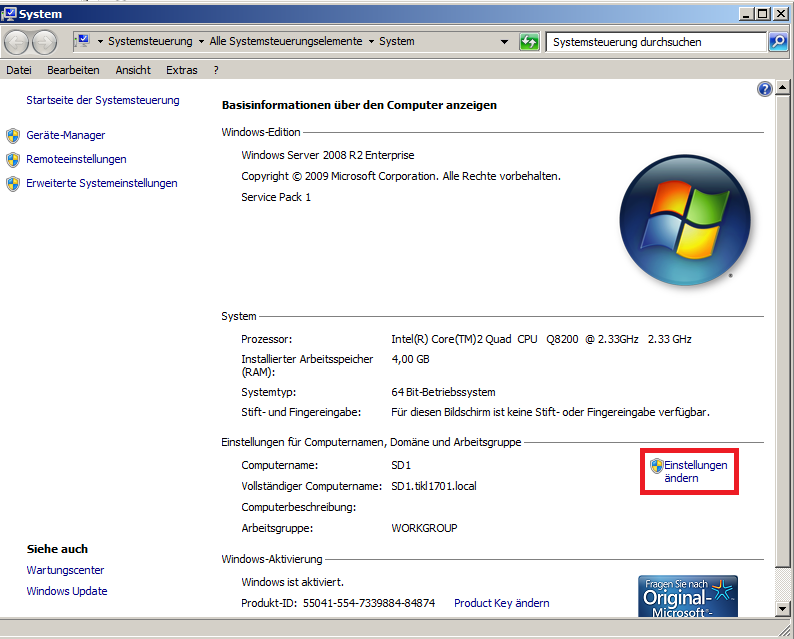
\includegraphics[width=14cm]{Bilder/001(Kasten)}\\
\newpage
Daraufhin erscheint folgender Dialog:

	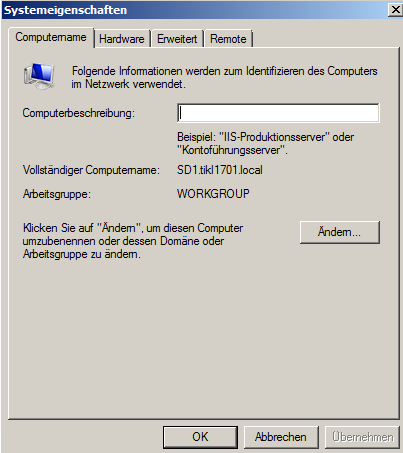
\includegraphics[height=7cm]{Bilder/002}
	
Hier kann man mit der Schaltfläche \emph{ändern} einen anderen Computernamen angeben.\\

	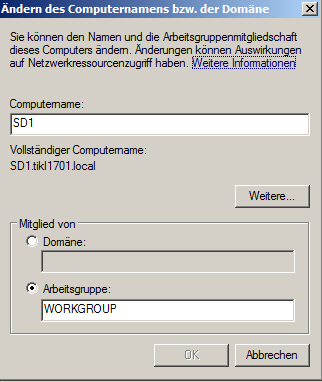
\includegraphics[height=7cm]{Bilder/003}
	
Die Arbeitsgruppe kann auf dem Standard belassen werden da dies eh angepasst wird bei der Installation des Domain Controllers.\\
Als nächstes muss man die IP-Einstellungen der Netzwerkkarte überprüfen, da ein Domain Controller eine feste IP benötigt. Die Einstellungen findet man z.B. unter \emph{Systemsteuerung \ding{221} Alle Systemsteuerungselemente \ding{221} Netzwerk- und Freigabecenter}, dort den Netzwerkadapter suchen und im rechte Maustasten Menü \emph{Eigenschaften} wählen. Dort \emph{Internetprotokoll Version 4 (TCP/IPv4)} auswählen und auf die Schaltfläche \emph{Eigenschaften} klicken.\\ %\ding{221} is one of the left arrows from pifont

	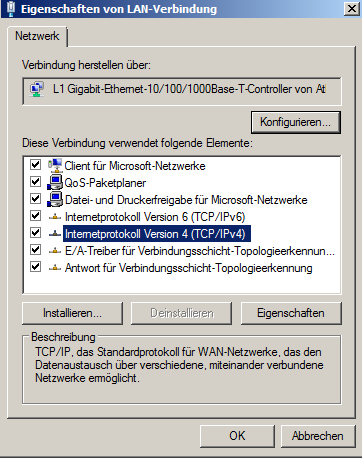
\includegraphics[height=7cm]{Bilder/004}\\
	
In dem folgenden Dialog kann man dann die IP-Adresse des Rechners fest. 

	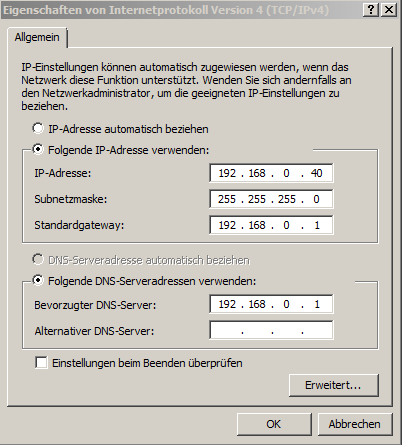
\includegraphics[height=7cm]{Bilder/005}\\
	
Dazu stellt man den Radiobutton auf \emph{Folgende IP-Adresse verwenden} und gibt dann eine in dem lokalen Netzwerk von keinem anderen Rechner benutzte IP-Adresse an, mit der passenden Subnetzmaske. als Standardgateway dient üblicherweise der Netzwerkrouter. Den DNS-Server muss man nun auch von Hand eingeben, dieser läuft üblicherweise auch auf dem Netzwerkrouter.\\
Damit wären die Vorarbeiten abgeschlosen, als nächstes wird die Active Directory-Domänendienste Rolle installiert.

\newpage
\section{Active Directory-Domänendienste installieren}
Zum installieren der Active Directory-Domänendienste öffnet man wie zum installieren jeder anderen Rolle auch den \emph{Server Manager}. Standardmäßig findet sich dieser in der Taskleiste. In der \emph{Rollenübersicht} wählt man \emph{Rollen hinzufügen} um die Rolle Active Directory-Domänendienste zu installieren.\\

	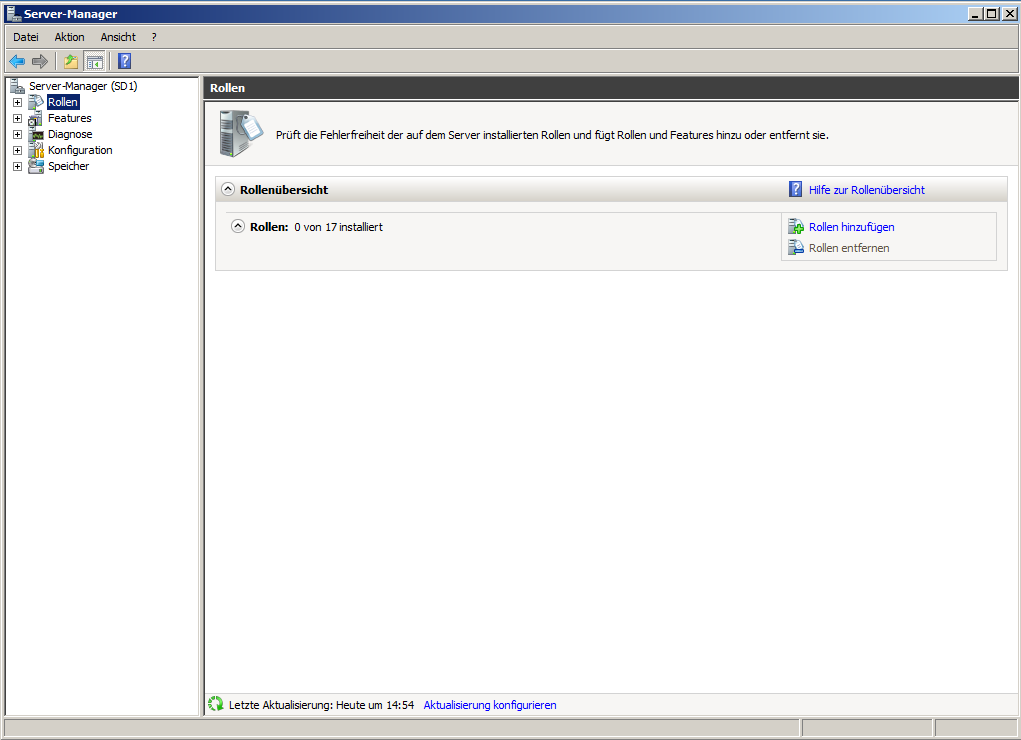
\includegraphics[width=14cm]{Bilder/006}\\
	
Den Bildschirm mit den Vorbemerkungen mit einem Klick auf \emph{Weiter} zur Kenntnis. Im \emph{Serverrollen auswählen} Dialog wählt man \emph{Active Directory-Domänendienste} aus und klickt auf \emph{Weiter}.\\

	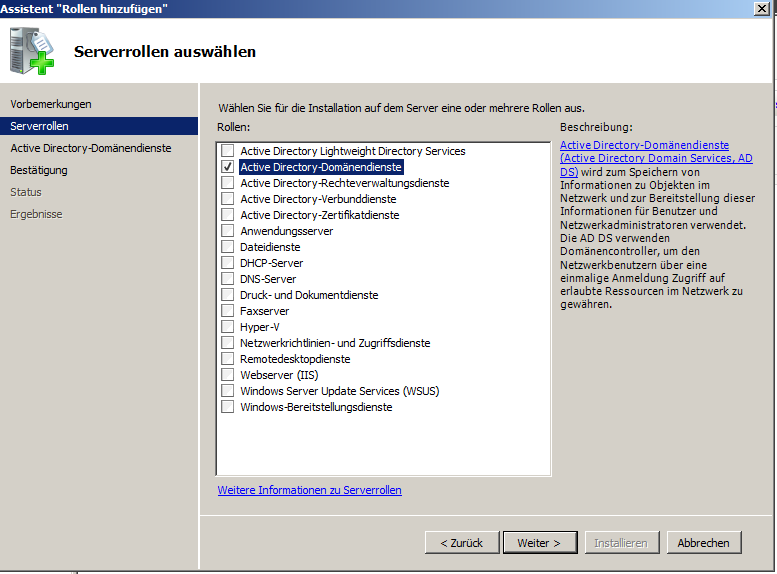
\includegraphics[height=9cm]{Bilder/008}\\
	
Die anderen Rollen die wir später noch installieren wollen können wir jetzt noch nicht installieren das Windows erst die Active Directory-Domänendienste Rolle komplett konfigurieren will bevor man weitere Rollen installieren darf.\\
 
 	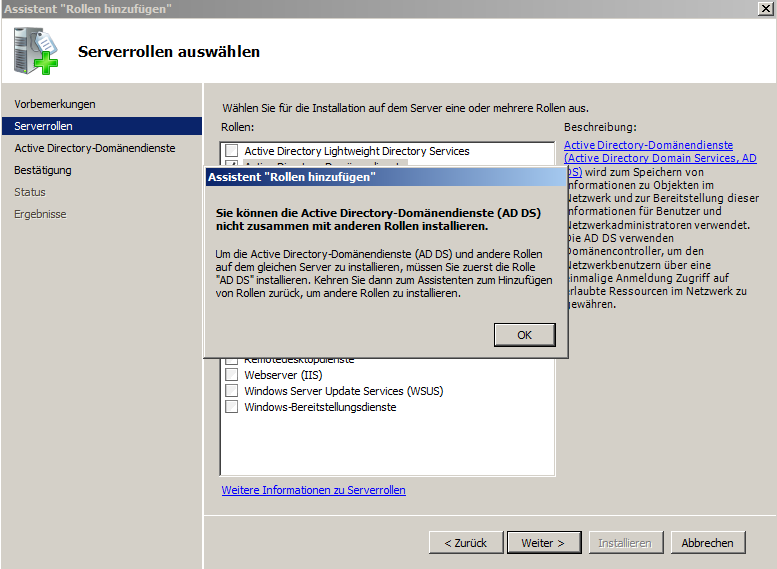
\includegraphics[height=9cm]{Bilder/009}\\
 	
Wenn es nicht bereits installiert ist will der Server Manager das benötigte .NET Framework 3.5.1 noch mitinstallieren. Den \emph{Einführung in die Active Directory-Domänendienste} Dialog durchlesen und mit einem Klick auf \emph{Weiter} zur Kenntnis nehmen. Daraufhin erhält man eine Übersicht der zu installierenden Rollen und Features, die man mit einem Klick auf \emph{Installieren} bestätigt.\\

 	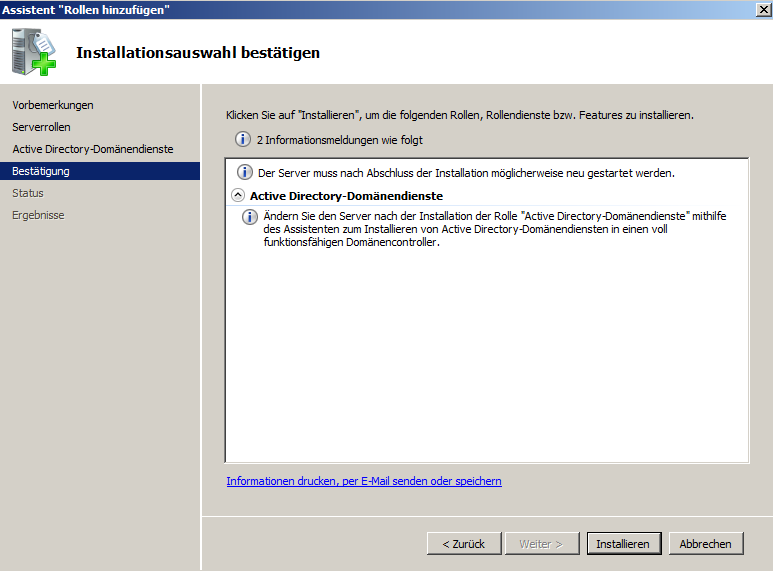
\includegraphics[height=9cm]{Bilder/011}\\
 
Daraufhin installiert Windows die Rollen und Features, dies kann einige Minuten in Anspruch nehmen. Zum Abschluss erscheint der \emph{Installationsergebnisse} Dialog, der für alles eine erfolgreiche Installation melden sollte. Danach muss der Active Directory-Domänendienst eingerichtet werden.
 
 \newpage
 \section{Active Directory-Domänendienste einrichten}
Um die Active Directory-Domänendienste einzurichten ruft man die dcpromo.exe auf.\\

	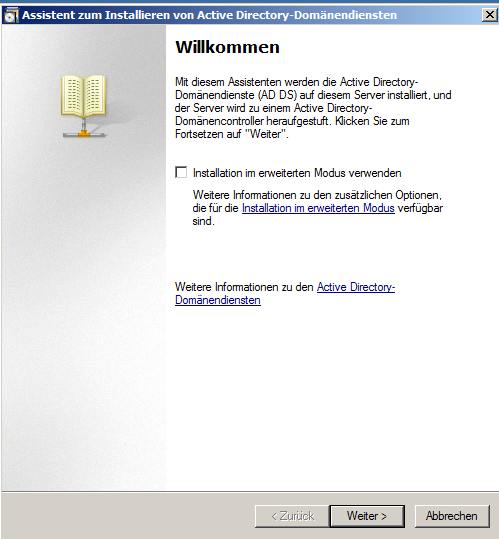
\includegraphics[height=7cm]{Bilder/014(dcpromo_exe01)}\\
	
Der Hinweis zur Betriebssystemkompatibilität kann von uns hier ignoriert werden, sollte aber trotzdem durchgelesen und dann mit \emph{Weiter} abgenickt werden. In dem darauffolgenden Dialog wählen wir \emph{Neue Domäne in neuer Gesamtstrutktur erstellen} da wir über keine bestehende Do,mäne verfügen die wir verwenden wollen.\\

	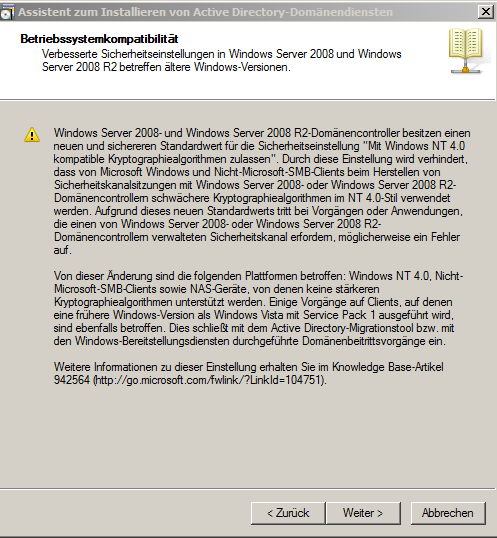
\includegraphics[height=7cm]{Bilder/015(dcpromo_exe02)}\\
	
Als nächstes muss der Fully Qualified Domain Name (\emph{FQDN}) der neuen Domäne angegeben werden. Da wir keine internetfähige Domäne verwalten wollen geben wir einen Namen an der auf \emph{.local} endet.\\

	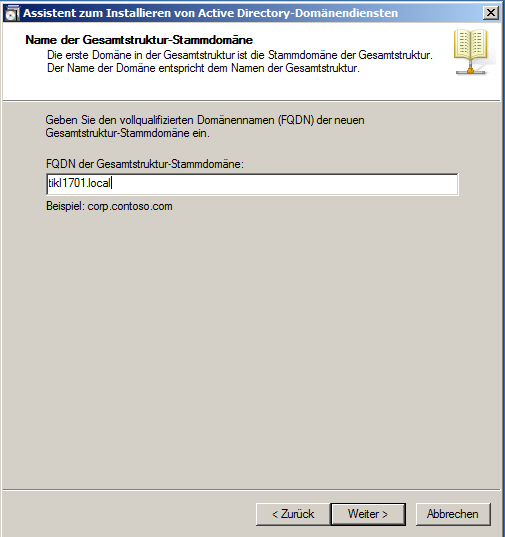
\includegraphics[height=7cm]{Bilder/017(dcpromo_exe04)}\\
		
Nach dem klicken auf \emph{Weiter} wird geprüft ob der angegebene Name schon verwendet wird. Als nächstes sollen wir die Funktionsebene der Gesamtstruktur festlegen. Da wir die Domäne komplett neu aufsetzen wählen wir das neueste verfügbare, also \emph{Windows Server 2008 R2}.\\

	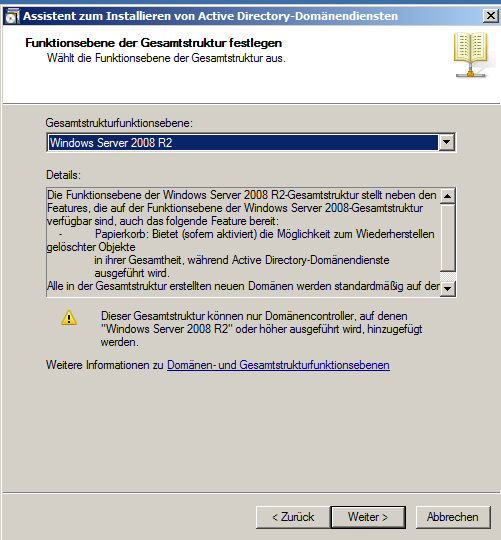
\includegraphics[height=7cm]{Bilder/019(dcpromo_exe06)}\\
	
Nach einem Klick auf \emph{Weiter} wird erst die vorhanden DNS-Konfiguration geprüft, danach erscheint der Dialog \emph{Weitere Domänencontrolleroptionen}.\\

	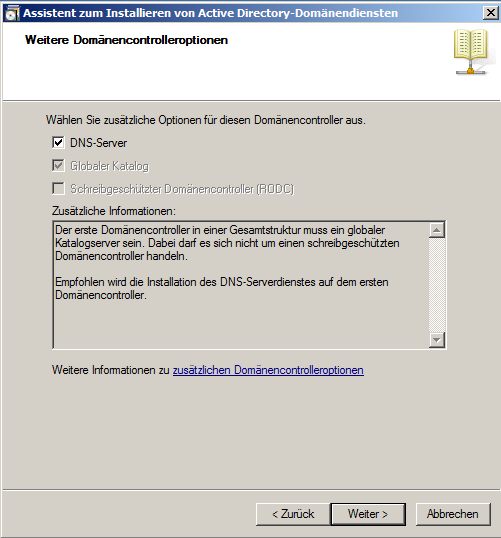
\includegraphics[height=7cm]{Bilder/021(dcpromo_exe08)}\\

Da wir später auch noch einen \emph{DNS-Server} aufsetzen wollen wählen wir diese Option aus. Da wir den ersten Domain Controller der Domäne einrichten muss die Option \emph{Globaler Katalog} zwingend aktiviert sein und darf auch nicht deaktiviert werden. Aus demselben Grund kann die Option \emph{Schreibgeschützer Domänencontroller (RODC)} nicht aktiviert werden.\\
Nach einem Klick auf \emph{Weiter} erscheint eine Fehlermeldung da wir den DNS-Server noch nicht eingerichtet haben und kein übergeordneter DNS-Server verfügbar ist.\\

	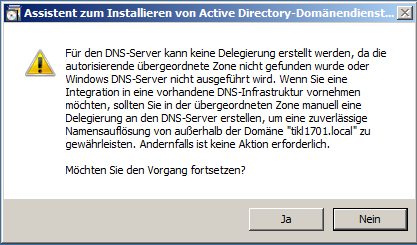
\includegraphics[height=7cm]{Bilder/022(dcpromo_exe09)}\\
	
Den Dialog mit \emph{Ja} bestätigen.\\
Danach wird nach den Speicherorten für Datanbank, Protokolldateien und SYSVOL gefragt. Da wir nichts an den Standardorten ändern wollen bestätigen wir das Ganze einfach mit \emph{Weiter}.\\
Danach müssen wir dem Administratorkonto für die Domäne ein Kennwort vergeben, nach den üblichen Richtlinien (mindestens 8 Stellen, mindestens 1 Buchstabe, mindestens 1 Zahl). Hier sollte ein möglichst sicheres Kennwort gewählt werden. Dies eintragen und nochmal zur Bestätigung eintragen, danach \emph{Weiter} wählen.\\
Nun wird eine Zusammenfassung unserer Einstellungen angezeigt bevor diese ausgeführt werden. Hier könnte man diese Einstellungen durch klicken auf \emph{Einstellungen exportieren} falls wir dieselben Einstellungen auf mehreren Rechnern ausführen wollen würden. Aber dies ist bei dem primären Domaincontroller nicht allzu sinnvoll und auch nicht Ziel diese Dokumentation. Nach der Bestätigung mit \emph{Weiter} richtet Windows den Domänencontroller ein. Dies kann einige Minuten in Anspruch nehmen.\\
Sobald alles eingerichtet ist beendet man den Assistenten mit einem Klick auf \emph{Fertig stellen}, danach muss man den Server neu starten. Dies schließt auch die Installation des Active Directory-Domänendienste ab.

\newpage
\section{DNS-Server installieren und einrichten}
Zuerst einmal muss hierfür die DNS-Server Rolle im \emph{Server Manager} installiert werden. Dies geht analog zur Installation der Active Directory-Domänendienste Rolle aus Kapitel 2. Danach öffnet man die DNS Einstellungen im Server Manager und klappt den Baum so lange auf bis man den Punkt \emph{Reverse-Lookupzonen} sieht.\\

	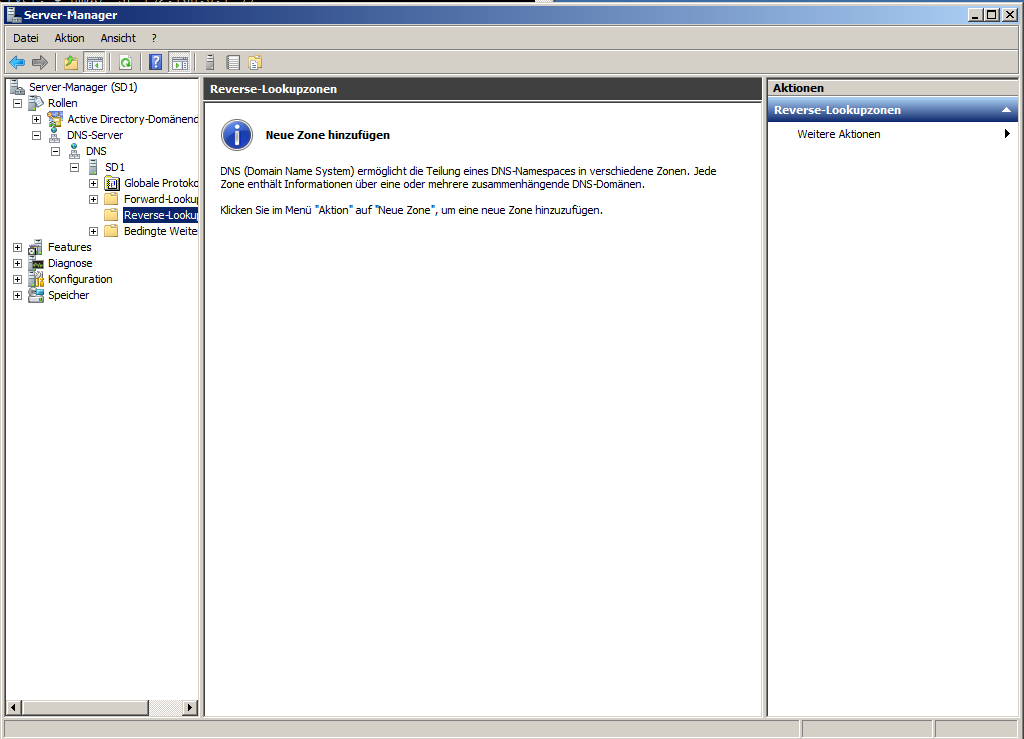
\includegraphics[height=9cm]{Bilder/029(DNS01)}\\

Um eine neue Reverse-Lookupzone zu erstellen wählt man diesen Punkt mit der rechten Maustaste an und wählt \emph{Neue Zone} aus.\\
Den Willkommensbildschirm nehmen wir mit der Auswahl von \emph{Weiter} zur Kenntnis. Als nächstens wählen wir die vorausgewählte Option \emph{Primäre Zone} da dies die erste (und vorerst die einzige) Zone ist die wir erstellen. Mit \emph{Weiter} bestätigen. Auch im nächsten Bildschirm wählen wir für die Zonenreplikation die vorausgewählte Option \emph{Auf allen Servern, die auf Domänencontrollern in dieser Domäne ausgeführt werden: \textit{Domänenname}} (in unserem Beispiel tikl1701.local). \emph{Weiter} führt auch hier... weiter. In unserem Beispiel arbeiten wir mit IPv4 Adressen, deswegen wählen wir im nächsten Bildschirm wieder die Voreinstellung \emph{IPv4 Reverse-Lookupzone}.\\
Die Auswahl von \emph{Weiter} führt wie fast immer zum nächsten Dialog in welchen nun der \emph{Name der Reverse-Lookupzone} angegeben werden soll.\\

	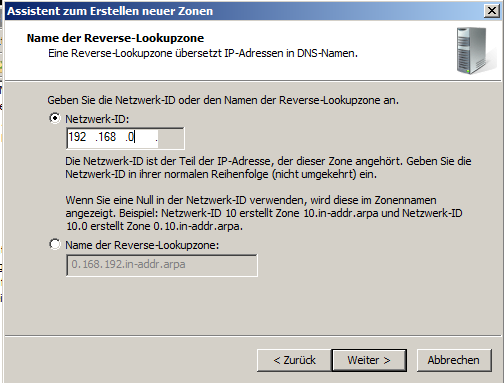
\includegraphics[height=7cm]{Bilder/034(DNS06)}\\
	
Hier muss nun die Netzwerk-ID angeben werden, also in unserem Beispiel die 192.168.0. Die Auswahl von \emph{Weiter} führt zu Dialog \emph{Dynamisches Update}. Hier wählen wir \emph{Nur sichere dynamische Updates zulassen} da dies die empfohlene Option für Active Directory ist.\\
Die Auswahl von \emph{Weiter} führt uns auch schon zum \emph{Fertigstellen des Assistenten} Dialogs, der nochmal die vorzunehmenden Einstellungen zusammenfasst. Dieser wird dann mit \emph{Fertig stellen} beendet.\\

	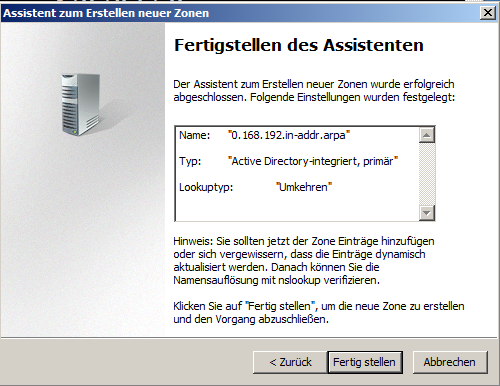
\includegraphics[height=7cm]{Bilder/036(DNS08)}\\

Als nächstes wählen wir im \emph{Server Manager} den eigenen Rechnernamen mit der rechten Maustaste aus und wählen dort \emph{Eigenschaften}. Hier kontrollieren wir ob im Reiter \emph{Weiterleitungen} der DNS-Server des Netzes für externe Anfragen eingetragen ist. Normalerweise wurde dies schon vom Assistenten erledigt, falls nicht muss sie durch Klick auf \emph{Bearbeiten} eingetragen werden.\\

	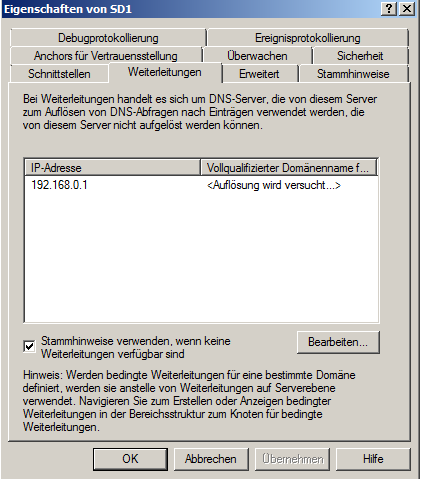
\includegraphics[height=7cm]{Bilder/038(DNS10)}\\

Somit ist die Einrichtung des DNS-Servers abgeschlossen, als nächstes wird der DHCP-Server eingerichtet.

\newpage
\section{DHCP-Server installieren und einrichten}
Zuerst einmal muss die DHCP-Server Rolle mit dem \emph{Server Manager} installiert werden, analog zur Active Directory-Domänendienste Rolle in Kapitel 2.\\

	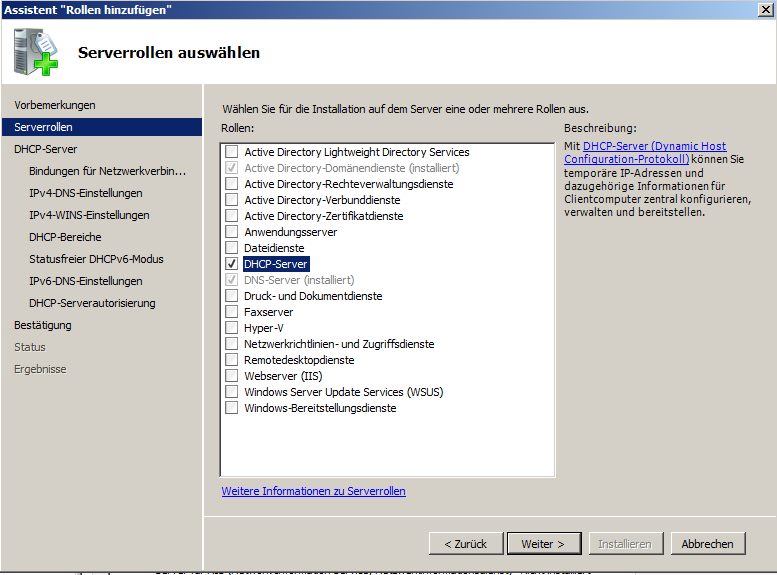
\includegraphics[height=9cm]{Bilder/039(DHCP01)}\\

Die allgemeinen Hinweise zu DHCP-Servern, ebenso wie die vorherige Auswahl, bestätigen wir mit einem Klick auf \emph{Weiter}. Als nächstes müssen wir den Namen unserer Domäne angeben
\end{document}
